\documentclass[../thesis.tex]{subfiles}

\begin{document}
Το Flutter είναι ένα framework ανάπτυξης cross-platform εφαρμογών για Android, iOS και Web που δημιουργήθηκε και αναπτύσσεται από την Google.
Η Google παρουσίασε για πρώτη φορά το 2015 μία πειραματική έκδοση του Flutter υπό την ονομασία “Sky”, αναφέροντας ως πρωταρχικό στόχο του νέου αυτού framework την εύκολη και γρήγορη ανάπτυξη αποδοτικών mobile εφαρμογών.
Το Flutter είναι άρρηκτα συνδεδεμένο με την γλώσσα προγραμματισμού Dart, η οποία αναπτύσσεται επίσης από την Google.

Ως framework ανάπτυξης cross-platform εφαρμογών, το Flutter καθιστά δυνατή την συγγραφή ενιαίου κώδικα για όλες τις υποστηριζόμενες πλατφόρμες.
Ο προγραμματιστής αρκεί να αναπτύξει την εφαρμογή μία φορά στη γλώσσα Dart,
αγνοώντας σε μεγάλο βαθμό τις λεπτομέρειες υλοποίησης της κάθε πλατφόρμας,
και όλες οι διαδικασίες που είναι απαραίτητες για την λειτουργία της εφαρμογής στη εκάστοτε πλατφόρμα γίνονται αυτόματα.
Συγκεκριμένα, μέσω του Flutter SDK ο κώδικας Dart που περιλαμβάνει την λογική και το UI της εφαρμογής μεταγλωττίζεται σε native machine code (πχ. ARM για κινητές συσκευές)

\section{Cross-platform}
Η cross-platform λειτουργία επιτυγχάνεται εν μέρει μέσα από την συμπερίληψη στο Flutter ειδικού rendering engine (Skia/Impeller) ο οποίος χειρίζεται εξ ολοκλήρου την σωστή εμφάνιση των στοιχείων του UI ανεξαρτήτως της πλατφόρμας.
Έτσι εφαρμογές Flutter δεν χρησιμοποιούν τα native UI components του κάθε λογισμικού συστήματος, αλλά αντιθέτως «ζωγραφίζουν» τα δικά τους components πάνω σε έναν καμβά, pixel ανά pixel.
Αυτή η μέθοδος απεικόνισης προσφέρει περισσότερη ομοιομορφία στην εμφάνιση των εφαρμογών σε όλες τις πλατφόρμες, ξεχωρίζοντας το Flutter από άλλα frameworks όπως το React Native (το οποίο αποτελεί τον κύριο ανταγωνιστή του Flutter στον τομέα των cross-platform εφαρμογών).

\section{Αρχιτεκτονική}
Μια εφαρμογή Flutter αποτελείται από τα παρακάτω αρχιτεκτονικά επίπεδα:
\begin{figure}
    \centering
    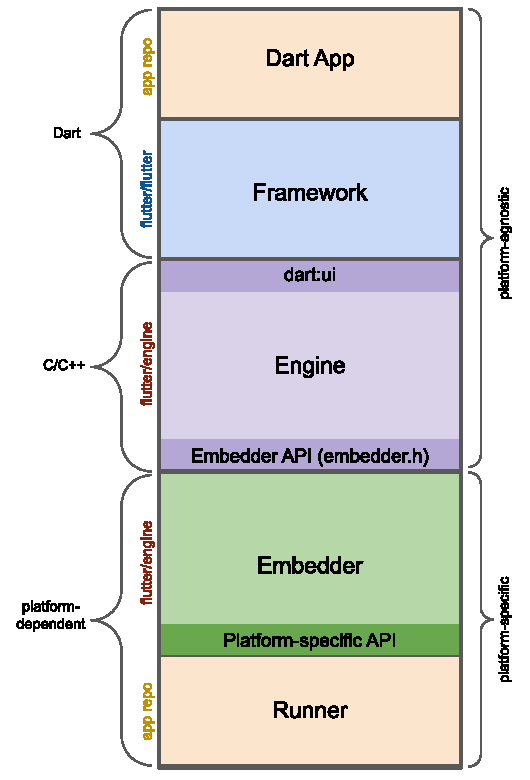
\includegraphics[scale=0.7]{flutter_architecture}
\end{figure}
\begin{itemize}
    \item \textbf{Runner και Embedder}: Αποτελούν τη βάση της εφαρμογής και τον δίαυλο επικοινωνίας με το λογισμικό σύστημα. Είναι υπεύθυνα για την εκκίνηση της εφαρμογής, την ενημέρωσή της σχετικά με όλα τα system events, και την δημιουργία του βάθρου πάνω στο οποίο ο engine θα εμφανίσει τα περιεχόμενα της εφαρμογής. Εφόσον τα δύο αυτά επίπεδα είναι άμεσα συνυφασμένα με το λογισμικό, ο σχετικός κώδικας είναι προσαρμοσμένος ειδικά για την εκάστοτε πλατφόρμα (πχ. χρησιμοποιείται Java/C++ για Android, και Objective-C για iOS)
    \item \textbf{Engine}: Αποτελεί τον πυρήνα μίας εφαρμογής Flutter. Συνιστάται από ένα runtime το οποίο εκτελεί τον κώδικα της εφαρμογής που είναι γραμμένος σε Dart, και χειρίζεται παράλληλα την εμφάνιση όλων των γραφικών στην οθόνη. Εφόσον επικοινωνεί με το λογισμικό διαμέσου του embedder, ο engine είναι ανεξάρτητος της πλατφόρμας (platform-agnostic)
    \item \textbf{Framework και Dart App}: Αποτελούν το υψηλού επιπέδου τμήμα της εφαρμογής. Το Flutter framework περιέχει όλα τα components με τα οποία ο προγραμματιστής θα συνθέσει την εφαρμογή, καθώς και εργαλεία για τον χειρισμό υπηρεσιών όπως τα animations και το gesture detection. Το τελευταίο επίπεδο είναι το μέρος της εφαρμογής που σχεδιάζεται εξ ολοκλήρου από τον developer, και περιέχει όλη την λογική μαζί με το UI, όπως αυτά έχουν οριστεί από τον προγραμματιστή. Τόσο το Flutter framework όσο και ο κώδικας της εφαρμογής είναι γραμμένα στη γλώσσα Dart.
\end{itemize}

\section{Widgets}
Η βασική μονάδα όλων των στοιχείων του UI στο Flutter είναι το widget.
Ένα widget περιγράφει ένα μέρος του UI της εφαρμογής, όπως ένα κουμπί, κείμενο, ή εικονίδιο.
Πέρα από τα εμφανή λειτουργικά στοιχεία, στα widgets συμπεριλαμβάνονται και στοιχεία που ελέγχουν την διάταξη/layout της εφαρμογής, όπως τα widget στοίχισης, padding, και δημιουργίας στηλών/γραμμών.
Η εφαρμογή έχει ως ρίζα ένα βασικό widget το οποίο αποτελεί το υπόβαθρο του συνόλου της διεπαφής, και όλα τα στοιχεία του UI δομούνται μέσα από την σύνθεση και την εμφώλευση απλών widget.
Έτσι όλες οι εφαρμογές Flutter έχουν την δομή ενός δέντρου, με το κάθε widget να διαθέτει έναν γονιό/parent (το widget μέσα στο οποίο είναι εμφωλευμένο) και ενδεχόμενα παιδιά/children (τα widget τα οποία περιέχει).

\end{document}